%% abtex2-modelo-relatorio-tecnico.tex, v-1.7.1 laurocesar
%% Copyright 2012-2013 by abnTeX2 group at http://abntex2.googlecode.com/ 
%%
%% This work may be distributed and/or modified under the
%% conditions of the LaTeX Project Public License, either version 1.3
%% of this license or (at your option) any later version.
%% The latest version of this license is in
%%   http://www.latex-project.org/lppl.txt
%% and version 1.3 or later is part of all distributions of LaTeX
%% version 2005/12/01 or later.
%%
%% This work has the LPPL maintenance status `maintained'.
%% 
%% The Current Maintainer of this work is the abnTeX2 team, led
%% by Lauro César Araujo. Further information are available on 
%% http://abntex2.googlecode.com/
%%
%% This work consists of the files abntex2-modelo-relatorio-tecnico.tex,
%% abntex2-modelo-include-comandos and abntex2-modelo-references.bib
%%

% ------------------------------------------------------------------------
% ------------------------------------------------------------------------
% abnTeX2: Modelo de Relatório Técnico/Acadêmico em conformidade com 
% ABNT NBR 10719:2011 Informação e documentação - Relatório técnico e/ou
% científico - Apresentação
% ------------------------------------------------------------------------ 
% ------------------------------------------------------------------------

% Alterado por Rodrigo Campiolo para apresentação de relatórios na disciplina
% de Redes de Computadores II do Bacharelado em Ciência da Computação da UTFPR-CM.


\documentclass[
	% -- opções da classe memoir --
	12pt,				% tamanho da fonte
	%openright,			% capítulos começam em pág ímpar (insere página vazia caso preciso)
	oneside,   	        % para impressão em verso e anverso use twoside. Oposto a oneside
	a4paper,			% tamanho do papel. 
	% -- opções da classe abntex2 --
	%chapter=TITLE,		% títulos de capítulos convertidos em letras maiúsculas
	%section=TITLE,		% títulos de seções convertidos em letras maiúsculas
	%subsection=TITLE,	% títulos de subseções convertidos em letras maiúsculas
	%subsubsection=TITLE,% títulos de subsubseções convertidos em letras maiúsculas
	% -- opções do pacote babel --
	english,			% idioma adicional para hifenização
	french,				% idioma adicional para hifenização
	spanish,			% idioma adicional para hifenização
	brazil,				% o último idioma é o principal do documento
	]{pacotes/abntex2}


% ---
% PACOTES
% ---

% ---
% Pacotes fundamentais 
% ---
\usepackage{cmap}				% Mapear caracteres especiais no PDF
\usepackage{lmodern}			% Usa a fonte Latin Modern
\usepackage[T1]{fontenc}		% Selecao de codigos de fonte.
\usepackage[utf8]{inputenc}		% Codificacao do documento (conversão automática dos acentos)
\usepackage{indentfirst}		% Indenta o primeiro parágrafo de cada seção.
\usepackage{color}				% Controle das cores
\usepackage{graphicx}			% Inclusão de gráficos
% ---

% ---
% Pacotes adicionais, usados no anexo do modelo de folha de identificação
% ---
\usepackage{multicol}
\usepackage{multirow}
% ---
	
% ---
% Pacotes adicionais, usados apenas no âmbito do Modelo Canônico do abnteX2
% ---
\usepackage{lipsum}				% para geração de dummy text
% ---

% ---
% Pacotes de citações
% ---
\usepackage[brazilian,hyperpageref]{backref}	 % Paginas com as citações na bibl
\usepackage[alf]{pacotes/abntex2cite}	% Citações padrão ABNT
\usepackage{comment}

% ---
% Meus pacotes
% ---
\usepackage{float}
\usepackage{array}
% ---

% --- 
% CONFIGURAÇÕES DE PACOTES
% --- 

% ---
% Configurações do pacote backref
% Usado sem a opção hyperpageref de backref
\renewcommand{\backrefpagesname}{Citado na(s) página(s):~}
% Texto padrão antes do número das páginas
\renewcommand{\backref}{}
% Define os textos da citação
\renewcommand*{\backrefalt}[4]{
	\ifcase #1 %
		Nenhuma citação no texto.%
	\or
		Citado na página #2.%
	\else
		Citado #1 vezes nas páginas #2.%
	\fi}%
% ---

% ---
% Informações de dados para CAPA e FOLHA DE ROSTO
% ---
\titulo{Simulação de Algoritmos de Escalonamento}
\autor{Hendrick Felipe Scheifer\\João Victor Briganti\\Luiz Gustavo Takeda}
\local{Campo Mourão}
\data{Novembro / 2024}
\instituicao{%
  Universidade Tecnológica Federal do Paraná -- UTFPR
  \par
  Departamento Acadêmico de Computação -- DACOM
  \par
  Bacharelado em Ciência da Computação -- BCC
}
\tipotrabalho{Relatório técnico}
% O preambulo deve conter o tipo do trabalho, o objetivo, 
% o nome da instituição e a área de concentração 
\preambulo{Relatório técnico de atividade prática solicitado pelo professor Rodrigo Campiolo na disciplina de Redes de Computadores II do Bacharelado em Ciência da Computação da Universidade Tecnológica Federal do Paraná.}
% ---

% ---
% Configurações de aparência do PDF final

% alterando o aspecto da cor azul
\definecolor{blue}{RGB}{41,5,195}

% informações do PDF
\makeatletter
\hypersetup{
     	%pagebackref=true,
		pdftitle={\@title}, 
		pdfauthor={\@author},
    	pdfsubject={\imprimirpreambulo},
	    pdfcreator={LaTeX with abnTeX2},
		pdfkeywords={abnt}{latex}{abntex}{abntex2}{relatório técnico}, 
		colorlinks=true,       		% false: boxed links; true: colored links
    	linkcolor=blue,          	% color of internal links
    	citecolor=blue,        		% color of links to bibliography
    	filecolor=magenta,      		% color of file links
		urlcolor=blue,
		bookmarksdepth=4
}
\makeatother
% --- 

% --- 
% Espaçamentos entre linhas e parágrafos 
% --- 

% O tamanho do parágrafo é dado por:
\setlength{\parindent}{1.3cm}

% Controle do espaçamento entre um parágrafo e outro:
\setlength{\parskip}{0.2cm}  % tente também \onelineskip

% ---
% compila o indice
% ---
\makeindex
% ---

% Omite a numeração de capítulos
\renewcommand*\thesection{\arabic{section}}



% ----
% Início do documento
% ----
\begin{document}

% Retira espaço extra obsoleto entre as frases.
\frenchspacing 

% ----------------------------------------------------------
% ELEMENTOS PRÉ-TEXTUAIS
% ----------------------------------------------------------
% \pretextual

% ---
% Capa
% ---
%\imprimircapa
% ---

% ---
% Folha de rosto
% (o * indica que haverá a ficha bibliográfica)
% ---
\imprimirfolhaderosto
% ---


% ---
% RESUMO
% ---

% resumo na língua vernácula (obrigatório)
\begin{resumo}
FAZER
 \vspace{\onelineskip}
    
 \noindent
 \textbf{Palavras-chave}: ESCOLHER.
\end{resumo}
% ---

% ---
% inserir lista de ilustrações
% ---
%\pdfbookmark[0]{\listfigurename}{lof}
%\listoffigures*
%\cleardoublepage
% ---

% ---
% inserir lista de tabelas
% ---
%\pdfbookmark[0]{\listtablename}{lot}
%\listoftables*
%\cleardoublepage
% ---

% ---
% inserir lista de abreviaturas e siglas
% ---
%\begin{siglas}
%  \item[IP] Internet Protocol
%  \item[TCP] Transmission Control Protocol
%  \item[UDP] User Datagram Protocol
%\end{siglas}
% ---

% ---
% inserir o sumario
% ---
\pdfbookmark[0]{\contentsname}{toc}
\tableofcontents*
\cleardoublepage
% ---

% ----------------------------------------------------------
% ELEMENTOS TEXTUAIS
% ----------------------------------------------------------
\textual

\makeatletter
\renewcommand{\chapter}{\@gobbletwo}
\makeatother

\section{Introdução}
\label{sec:introducao}

\section{Objetivos}
\label{sec:objetivos}

\section{Fundamentação}
\label{sec:fundamentacao}

\section{Materiais}
\label{sec:materiais}

Simulador OS Sim na versão 1.2.

\section{Procedimentos e Resultados}
\label{sec:procedimentos}

O simulador OS Sim foi utilizado para analisar tempos e métricas de execução, avaliando o impacto de diferentes estratégias no escalonamento de processos. Esse estudo permitiu observar como cada algoritmo lida com a distribuição de tarefas, afetando a eficiência e o desempenho do sistema.

\subsection{FCFS (\textit{First-Come, First-Served})}
\label{subsec:fcfs}

O primeiro algoritmo analisado foi o FCFS, um dos algoritmos de escalonamento mais simples, ele funciona da seguinte maneira o processo a chegar e o primeiro a ser atendido, o segundo a chegar e o segundo a ser atendido, o terceiro a chegar e o terceiro a ser atendido e assim sucessivamente~\cite{maziero2019}. 

\subsubsection{FCFS \textit{First-Come, First-Served} Monoprogramação}
\label{subsubsec:mono_fcfs}

A primeira versão simulada deste algoritmo se deu de maneira monoprogramada, na prática, isso significa que apenas um programa pode estar na memória e executando na CPU ao mesmo tempo, dessa forma processos que realizam chamadas de E/S (Entrada/Saída) não podem ser colocados em estado de bloqueado, pois não há como trazer outro processo a memória para executar de maneira concorrente ao primeiro processo em execução. Desse modo, neste ambiente o programa que entrar em execução precisa ser levado até o final, mesmo que entre em estado de bloqueado~\cite{tanenbaum2016}.

A Figura~\ref{fig:fcfs-mono} apresenta o diagrama de Grant com o período de execução de cada processo. Os períodos em azul simbolizam a execução na CPU enquanto os amarelos são períodos de execução de E/S.

\begin{figure}[H]
  \centering
  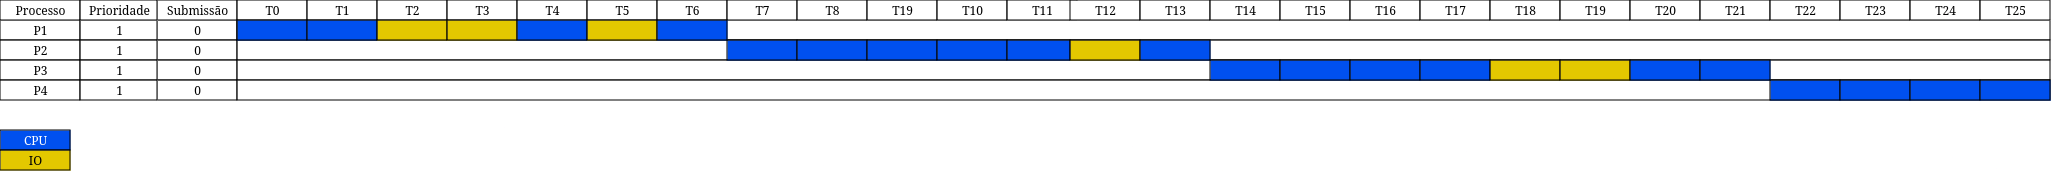
\includegraphics[scale=0.20]{figuras/ex1/fifo-mono.png}
  \caption{Diagrama de Grant do algoritmo FCFS em um ambiente monoprogramado.}
  \label{fig:fcfs-mono}
\end{figure}

A Figura~\ref{fig:table-fcfs-mono} apresenta uma tabela com informações de execução deste algoritmo. O tempo de criação do processo e o seu tempo de execução aumentaram conforme a posição do processo na fila, o fato de alguns processos não estarem utilizando a CPU (\textit{Central Processing Unit}) em  alguns momentos e mesmo assim consumindo seu tempo, acaba degradando bastante a execução dos processos de maneira geral.

\begin{figure}[H]
  \centering
  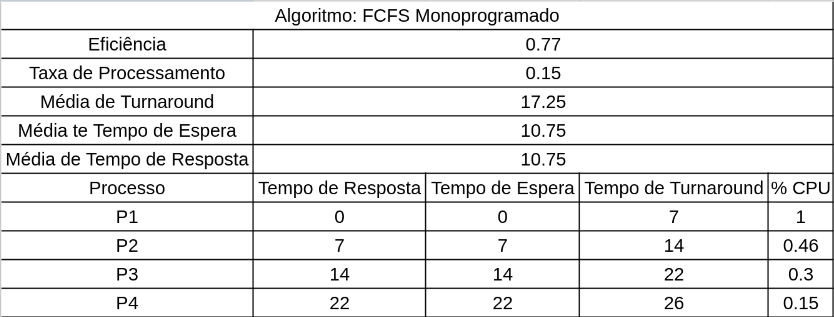
\includegraphics[scale=0.5]{figuras/ex1/table-fifo-mono.png}
  \caption{Tabela com informações de execução do FCFS em um ambiente monoprogramado.}
  \label{fig:table-fcfs-mono}
\end{figure}

\subsubsection{FCFS \textit{First-Come, First-Served} Multiprogramação}
\label{subsubsec:multi_fcfs}

Nesta segunda versão o algoritmo está em maneira multiprogramada, o que significa que mais de um programa pode estar na memória, o que vai permitir uma execução concorrente entre os processos. Desse modo, processos que realizam chamadas de E/S podem ser colocados no estado de bloqueado e passarem sua vez para que outro processo faça uso da CPU. Neste caso, processos que perdem sua vez na CPU, são colocados ao final da fila. 

A Figura~\ref{fig:fcfs-multi} apresenta o diagrama de Grant que ilustra os períodos de execução de cada processo.

\begin{figure}[H]
  \centering
  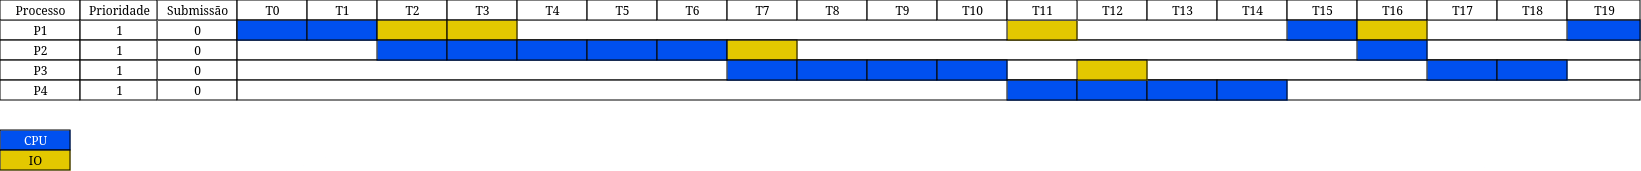
\includegraphics[scale=0.20]{figuras/ex1/fifo-multi.png}
  \caption{Diagrama de Grant do algoritmo FCFS em um ambiente multiprogramado.}
  \label{fig:fcfs-multi}
\end{figure}

A Figura~\ref{fig:table-fcfs-mono} apresenta uma tabela com informações de execução deste algoritmo. É possível perceber que este algoritmo, diferente de sua versão monoprogramada, faz um uso mais eficiente da CPU, pois em nenhum momento ela fica parada, porém, nesta versão do algoritmo processos que realizam E/S acabam sendo penalizados sendo colocados no final da fila.

\begin{figure}[H]
  \centering
  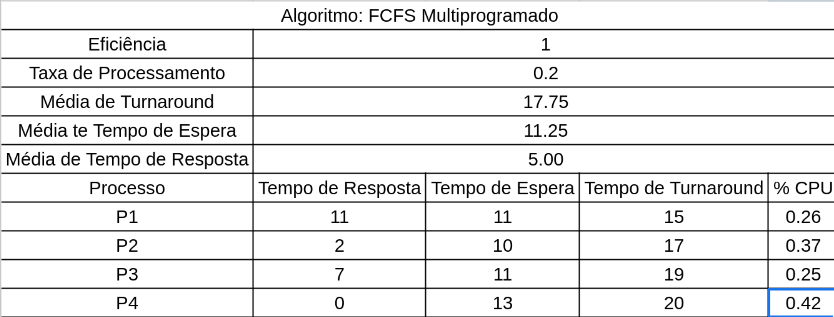
\includegraphics[scale=0.5]{figuras/ex1/table-fifo-multi.png}
  \caption{Tabela com informações de execução do algoritmo FCFS em um ambiente multiprogramado.}
  \label{fig:table-fcfs-multi}
\end{figure}

\subsection{Prioridade}
\label{subsec:prio}

O segundo algoritmo analisado foi o de prioridades, existem diferentes formas de se implementar esse algoritmo, no caso a escolhida pelo simulador é a de prioridades fixas. O algoritmo de prioridades fixas trabalha com a ideia de que cada processo possui uma prioridade associada, que não se altera ao longo da execução. Nesta sessão são analisadas duas variantes desse algoritmo, sua versão preemptiva e sua versão não preemptiva~\cite{maziero2019}.

\subsubsection{Prioridade Estática Não Preemptiva}
\label{subsubsec:prio_sem_preemp}

A preempção dentro de Sistemas Operacionais, está relacionada a retirar um processo que está atualmente executando da CPU para dar espaço para que outro processo execute. Quando está se falando de um algoritmo de prioridade não preemptivo, isso significa que a partir do momento que um processo começou a executar, ele não será retirado de lá, ao menos que ele realize uma operação de E/S ou ele finalize sua execução, seja ela uma finalização normal ou devido a um erro~\cite{maziero2019}.

Neste algoritmo de prioridade estática não preemptiva, o que ocorre é que o escalonador ao se deparar com dois processos na fila de aptos, irá escolher aquele com maior prioridade. A Figura~\ref{fig:prio_sem_preemp} apresenta um diagrama de Grant que ilustra a execução deste algoritmo.

\begin{figure}[H]
  \centering
  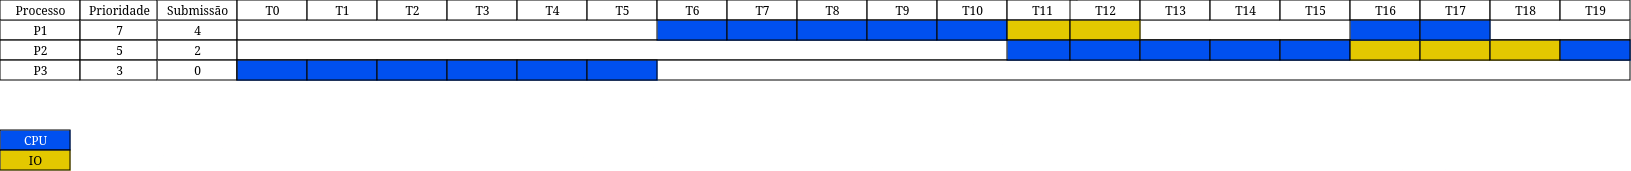
\includegraphics[scale=0.20]{figuras/ex2/prio_sem_preemp.png}
  \caption{Diagrama de Grant do algoritmo de Prioridade Estática Sem Preempção.}
  \label{fig:prio_sem_preemp}
\end{figure}

A Figura~\ref{fig:table_prio_sem_preemp} mostra uma tabela com algumas informações relacionadas a execução deste algoritmo. É possível perceber que está execução não teve 100\% eficiência, ficando abaixo do quer foi observado no algoritmo de FCFS Multiprogramada~\ref{subsubsec:multi_fcfs}, e de maneira geral a maneira como os processos foram selecionados se assemelha bastante a este algoritmo. Um dos grandes problemas dessa falta de preempção que pode ser observado é que processos mais prioritários por vezes precisam esperar processos menos prioritários terminarem sua execução, o que acaba sendo problemático se considerarmos que a proposta do algoritmo é o de processos mais prioritários primeiro e terminem antes.

\begin{figure}[H]
  \centering
  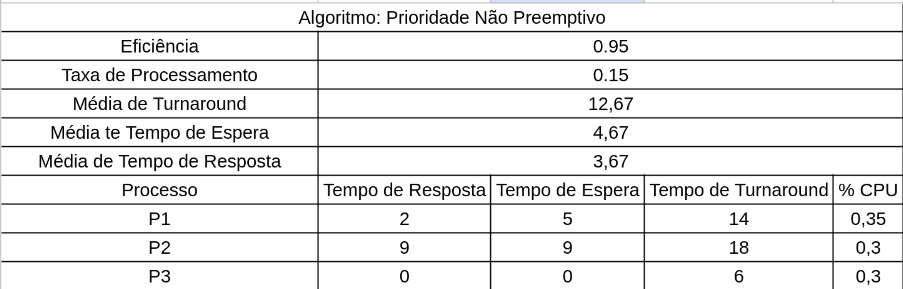
\includegraphics[scale=0.5]{figuras/ex2/table_prio_sem_preemp.png}
  \caption{Tabela com informações de execução do algoritmo de Prioridade Estática Sem Preempção.}
  \label{fig:table_prio_sem_preemp}
\end{figure}

\subsubsection{Prioridade Estática Preemptiva}
\label{subsubsec:prio_preemp}

Nesta versão do algoritmo temos o processo de preempção, isso significa que assim que um processo mais prioritário do que o que está sendo executado atualmente estiver apto, temos que o processo executando será removido da CPU e dará espaço para que este processo mais prioritário passe a executar. Isto ocorre até que um processo mais prioritário chegue na fila de aptos, ou que o processo executando finalize dando lugar a um processo menos prioritário.

 A Figura~\ref{fig:prio_preemp} apresenta um diagrama de Grant que ilustra a execução deste algoritmo.

\begin{figure}[H]
  \centering
  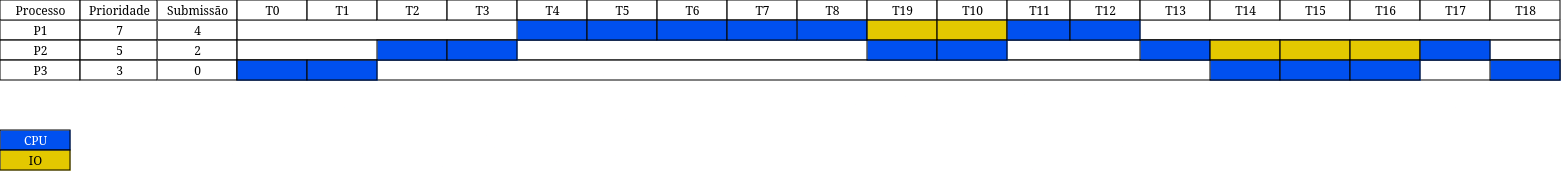
\includegraphics[scale=0.20]{figuras/ex2/prio_preemp.png}
  \caption{Diagrama de Grant do algoritmo de Prioridade Estática Preemptiva.}
  \label{fig:prio_preemp}
\end{figure}

A Figura~\ref{fig:table_prio_sem_preemp} mostra uma tabela com algumas informações relacionadas a execução deste algoritmo. Uma das características deste algoritmo está no fato de que o tempo de resposta customa ser menor, desde que o processo a ser executado seja o mais prioritário, na prática, isso significa que assim que um processo mais prioritário chegar na fila de aptos ele já será colocado em execução, o que diminui o tempo de resposta médio dos processos se comparado com sua versão não preemptiva. Uma das desvantagens deste algoritmo está no fato de que, se a todo instante chegar um processo que seja mais prioritário do que os já criados, ele será executado e os outros ficaram em espera, o que pode resultar em inanição.

\begin{figure}[H]
  \centering
  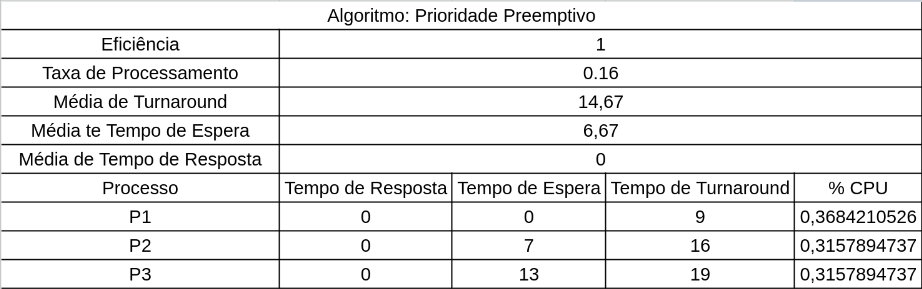
\includegraphics[scale=0.5]{figuras/ex2/table_prio_preemp.png}
  \caption{Tabela com informações de execução do algoritmo de Prioridade Estática Preemptiva.}
  \label{fig:table_prio_preemp}
\end{figure}

\subsection{Comparação Entre Algoritmos}
\label{subsec:algoritmos}


\section{Discussão dos Resultados}
\label{sec:discussao}

FAZER

\section{Conclusões}
\label{sec:conclusoes}

FAZER

% ----------------------------------------------------------
% ELEMENTOS PÓS-TEXTUAIS
% ----------------------------------------------------------
\postextual
% ----------------------------------------------------------
% Referências bibliográficas
% ----------------------------------------------------------
\renewcommand{\bibsection}{%
\section{\bibname}
\bibmark
%\ifnobibintoc\else
%\phantomsection
%\addcontentsline{toc}{section}{\bibname}
%\fi
\prebibhook}

\bibliography{abntex2-modelo-references}



% ----------------------------------------------------------
% Apêndices
% ----------------------------------------------------------

% ---
% Inicia os apêndices
% ---
\begin{apendicesenv}

% ----------------------------------------------------------
\section*{Apêndice A - Nome do Apêndice}
\addcontentsline{toc}{section}{Apêndice A - Nome do Apêndice}
% ----------------------------------------------------------

\end{apendicesenv}
% ---


% ----------------------------------------------------------
% Anexos
% ----------------------------------------------------------

% ---
% Inicia os anexos
% ---
\begin{anexosenv}

% ---
\section*{Anexo A - Nome do Anexo}
\addcontentsline{toc}{section}{Anexo A - Nome do Anexo}
% ---
\end{anexosenv}


\end{document}
